\documentclass[9pt]{article}
\usepackage{tikz}
\usetikzlibrary{arrows.meta,positioning,shapes.geometric,fit}
\usepackage[a4paper,margin=1in]{geometry}
\usepackage{amsmath}
\usepackage{graphicx}
\usepackage{subcaption}
\usepackage{multirow}
\usepackage{booktabs}
\usepackage{tabularx}
\usepackage{hyperref}
\usepackage{balance}
\usepackage[font=small,labelfont=bf]{caption}
\newcommand{\fakeparagraph}[1]{\vspace{3mm}\noindent\textbf{#1.}}
\newcommand{\fakepar}[1]{\fakeparagraph{#1}}
\tikzset{
  block/.style={
    rectangle,
    rounded corners,
    draw,
    align=center,
    minimum height=8mm,
    minimum width=28mm
  },
  decision/.style={
    diamond,
    draw,
    aspect=2,
    align=center,
    inner sep=1pt
  },
  line/.style={
    -{Latex[length=2mm]},
    thick
  }
}
\title{FeBEx: In-Network Deduplication for Federated LoRaWAN Backhaul Using P4 Programmable Switches}

\author{
Savitha Viswanadh Kandala\\
\small{\texttt{
viswanadh@u.nus.edu
}}
% School of Computing, National University of Singapore
\and
Rajashekar Reddy Chinthalapani\\
\small{\texttt{
rajashekar.c@u.nus.edu
}}
% School of Computing, National University of Singapore
}

\date{}

\begin{document}

\maketitle
\vspace{-8mm}
\begin{abstract}
Helium and similar federated LoRaWAN deployments solve the last-mile connectivity problem for IoT devices, but their architecture creates a fundamental inefficiency. When an end device transmits a single uplink packet, multiple geographically distributed hotspots may receive it and independently forward duplicate copies through the backhaul to cloud backends. While this redundancy improves reception reliability and coverage, it also inflates backhaul traffic, increases network cost, and wastes aggregation capacity.

We present FeBEx, a P4-programmable aggregation switch that moves packet deduplication from cloud backends into the network backhaul. FeBEx combines register-based duplicate detection with epoch-driven expiry, longest-prefix-match tenant steering, and packet cloning to preserve proof-of-coverage attribution. We implement FeBEx on a Mininet-BMv2 testbed and evaluate it across deployments with 50--500 devices and 5--50 hotspots. Our results show that FeBEx reduces redundant backhaul traffic by 50--90\% while preserving correct packet delivery, maintaining 100\% multi-tenant isolation, and enabling accurate payment attribution. We further identify practical operating guidelines, including register sizing of at least $4N$ entries and epoch intervals of 5--10 seconds. These results demonstrate that in-network deduplication is a practical and effective approach for reducing redundant backhaul traffic in federated LoRaWAN infrastructures. Find the code and implementation: \url{https://github.com/VIS-WA/FeBEx}.
\end{abstract}
\begingroup
\renewcommand{\thefootnote}{}
\footnotetext{\noindent\textbf{AI Tool Declaration:} We used ChatGPT (GPT-5.4 Thinking) and Claude (Opus 4.6 Extended) to generate ideas, improve wording and paragraph structure, refine technical explanations, assist with coding, and help draft and revise parts of this report, including figure captions and section-level writeups. We are responsible for the content, accuracy, and quality of the submitted work.}
\addtocounter{footnote}{-1}
\endgroup
\section{Introduction}

Helium and LoRaWAN networks have emerged as key infrastructure for low-power, wide-area connectivity in IoT deployments. However, the fundamental architecture of these networks creates a significant inefficiency: when a device broadcasts a single LoRa transmission, multiple geographically distributed hotspots may receive and independently forward the same packet to the cloud backend. This redundancy, while essential for reliability and network coverage, wastes precious backhaul bandwidth — a scarce and costly resource in network infrastructure.

Consider a typical Helium network deployment where hotspots are distributed across a city. When an IoT device transmits, perhaps five different hotspots receive the signal. Each hotspot independently sends a complete UDP/IP copy of the packet through the backhaul to a cloud data center. The cloud then performs packet deduplication in software, discarding the redundant copies. This results in a 5$\times$ multiplication of backhaul traffic for a single logical uplink, directly translating to increased bandwidth costs, higher latency, and reduced effective network capacity.

The conventional approach handles this duplication at the cloud tier --- a software post-processing step after packets have already consumed backhaul resources. FeBEx (Filtering in-network for Backhaul experiments) proposes a fundamental architectural shift: move deduplication into the network itself, specifically into a P4-programmable switch positioned as an aggregation point between hotspots and cloud backends.

\subsection{Motivation and Problem Statement}

The key insight is that deduplication can be solved efficiently in-network, at the edge where the switch can observe all incoming copies simultaneously. By implementing deduplication as a stateful forwarding action in a P4 programmable data plane, FeBEx achieves three critical benefits:

\begin{enumerate}
    \item \textbf{Backhaul bandwidth savings}: Duplicate packets are suppressed before egress, reducing backhaul traffic by 50-90\% depending on the degree of duplication.
    \item \textbf{Latency reduction}: The first copy reaches the backend immediately, without waiting for software-based cloud deduplication.
    \item \textbf{Payment accuracy}: A P4 clone session mirrors the first-forwarded packet to a separate Helium Cloud endpoint, enabling precise Proof-of-Coverage payments to the hotspot that legitimately delivered the uplink.
\end{enumerate}

\subsection{Research Questions}

This work addresses the following research questions:

\begin{enumerate}
    \item \textbf{Correctness}: Can an in-network deduplication filter correctly suppress true duplicates without falsely suppressing unique packets, even under high-collision hash conditions?
    \item \textbf{Efficiency}: How much backhaul bandwidth can in-network deduplication realistically save, and how does this scale with network topology and traffic patterns?
    \item \textbf{State requirements}: How large must the deduplication state (register arrays) be to achieve acceptable loss rates across different deployment scales?
    \item \textbf{Temporal sensitivity}: How sensitive is the deduplication mechanism to epoch rotation frequency, and is there a sweet spot that minimizes boundary leakage?
    \item \textbf{Scalability}: Does the approach maintain effectiveness across city-scale deployments with hundreds of devices and dozens of hotspots?
    \item \textbf{Multi-tenancy}: Can the P4 pipeline correctly handle multiple independent tenant networks through LPM-based traffic steering without cross-contamination?
\end{enumerate}

\subsection{Contributions}

This work presents:

\begin{enumerate}
    \item A complete P4-16 implementation of an in-network deduplication pipeline for LoRaWAN/Helium networks, running on BMv2 (v1model) with P4Runtime control plane.
    \item An evaluation framework (Mininet-based) that systematically explores parameter space: duplicate factors, register sizes, epoch intervals, network scales, and multi-tenant configurations.
    \item Seven comprehensive experiments (E1-E7) that validate correctness, measure realistic backhaul savings, and identify practical design parameters (e.g., register sizing, epoch interval tuning).
    \item An interactive visualization dashboard that animates the deduplication process in real-time across four city-scale scenarios.
    \item Empirical evidence that register-based deduplication with simple hash collision handling is viable for production-scale IoT network aggregation.
\end{enumerate}

\subsection{Paper Organization}

The remainder of this paper is organized as follows. Section~\ref{sec:related} surveys related work in network deduplication, P4 programming, and IoT backhaul optimization. Section~\ref{sec:background} provides necessary background on LoRaWAN, Helium networks, and P4 programmable switches. Section~\ref{sec:design} describes the FeBEx system architecture, including the P4 data plane, the control plane, and the evaluation topology. Section~\ref{sec:implementation} details the implementation, including packet format, P4 pipeline structure, and controller logic. Section~\ref{sec:evaluation} describes our experimental methodology and the seven experiments. Section~\ref{sec:results} presents empirical results and analysis for each experiment. Section~\ref{sec:discussion} discusses implications, limitations, and future work. Finally, Section~\ref{sec:conclusion} concludes.

% \section{Related Works}
\label{sec:related}

This work intersects several research areas: network deduplication, P4 programmable switching, IoT backhaul optimization, and in-network processing.

\subsection{Network Deduplication}

Packet deduplication at the network layer is well-studied. Traditional approaches operate at the cloud or core network layer. \textit{Cloud-based deduplication} is the standard in Helium and similar networks, where a centralized backend receives all copies and performs software-based duplicate detection using in-memory lookup tables or bloom filters. While simple and flexible, this approach wastes upstream bandwidth and processing resources.

\textit{Intermediate deduplication} has been explored in various contexts. For example, in wireless sensor networks, in-network packet aggregation and duplicate suppression have been used to reduce energy consumption~\cite{tada}. However, these approaches typically operate on lower-layer protocols (e.g., at the MAC layer) and do not address the specific challenges of heterogeneous IoT backhaul networks.

\textit{Middle-box deduplication} solutions (e.g., load balancers, NAT boxes) can perform stateful deduplication, but require dedicated middlebox infrastructure and do not integrate into the forwarding datapath. FeBEx differs by embedding deduplication as a first-class forwarding action in a P4-programmable switch, eliminating separate infrastructure.

\subsection{P4 and Programmable Networks}

P4~\cite{p4} is a domain-specific language for programming network packet forwarding in data plane devices. Since its introduction in 2014, P4 has enabled researchers and operators to implement custom network protocols and services without modifying underlying hardware or relying on vendor-specific instruction sets.

Notable P4-based services include:

\begin{enumerate}
    \item \textbf{Stateful packet processing}: Services like INT (In-band Network Telemetry)~\cite{int} use P4 registers and arithmetic to collect per-packet metrics. FeBEx applies similar register-based state to track deduplication keys.
    \item \textbf{Load balancing}: P4-based load balancers~\cite{conga,clove} use hash functions and port selection logic implemented in P4 pipelines. FeBEx similarly uses dual CRC32 hashing for key indexing and verification.
    \item \textbf{In-network aggregation}: Techniques like data aggregation in switches have been explored to reduce bandwidth in data center and wide-area networks~\cite{netcache}.
    \item \textbf{Multi-tenant isolation}: P4 pipelines can enforce tenant isolation through LPM-based forwarding and table-entry-based access control, as demonstrated in virtual network slicing systems.
\end{enumerate}

Our work applies P4 to a new domain (IoT backhaul deduplication) and validates practical design choices (register sizing, hash collision handling, epoch-based expiry) that may be applicable to other stateful P4 services.

\subsection{Hash-Based Deduplication}

Bloom filters and hash tables are classical approaches to deduplication. A naive approach stores the full packet or a cryptographic hash and performs exact-match lookup. However, this is expensive in switch memory.

FeBEx uses a two-level hash approach: a primary hash function selects the register index, and a second hash function serves as a verification key to disambiguate collisions. This is a well-known technique in hash table design~\cite{hashtables} and is adopted here to fit within typical P4 register constraints (typically 32-64 KB per switch).

Bloom filters offer probabilistic deduplication with tunable false-positive rates~\cite{bloomfilters}. FeBEx does not use Bloom filters directly; instead, it implements a deterministic hash table with overflow handling through register size tuning. This trades off some flexibility for simplicity and determinism in a P4 context.

\subsection{IoT and LoRaWAN Infrastructure}

LoRaWAN is a Low Power Wide Area Network (LPWAN) protocol standardized by the LoRa Alliance. Helium is a community-driven network operating at LoRaWAN frequencies.

Infrastructure challenges in LoRaWAN include:

\begin{enumerate}
    \item \textbf{Backhaul congestion}: As networks scale, the backhaul from gateways to cloud becomes a bottleneck, especially in dense urban deployments.
    \item \textbf{Packet loss}: Congestion and limited gateway capacity lead to packet loss, reducing network reliability.
    \item \textbf{Cost}: Backhaul bandwidth is expensive, especially for deployment in cost-sensitive regions.
    \item \textbf{Proof-of-Coverage}: In incentivized networks like Helium, gateways must be compensated based on coverage contribution. This requires accurate attribution of which gateway delivered a given packet.
\end{enumerate}

FeBEx directly addresses backhaul congestion and cost by moving deduplication from cloud to edge. It maintains Proof-of-Coverage accuracy through clone sessions that mirror authenticated receipts to the Helium Cloud.

\subsection{Edge Computing and Programmable Switches}

The emergence of programmable switches (Barefoot Tofino, NetronomeAgilio, etc.) has enabled a new class of \textit{edge services} --- stateful services running in the forwarding datapath rather than in separate appliances or cloud servers. Examples include:

\begin{enumerate}
    \item \textbf{Network monitoring and telemetry}: Switches can collect and aggregate statistics in-band~\cite{int}.
    \item \textbf{Consensus and coordination}: In-switch services have been used to implement distributed state machine replication~\cite{silkroad}.
    \item \textbf{Load balancing}: Switches can make intelligent forwarding decisions based on live server state~\cite{conga}.
\end{enumerate}

FeBEx is positioned in this space as an edge deduplication service. By implementing deduplication in the switch, we move a CPU-bound cloud operation into hardware-accelerated forwarding, reducing latency and cost.

\subsection{Summary and Positioning}

FeBEx is unique in combining:
\begin{enumerate}
    \item \textbf{Domain focus}: Specific to IoT/LoRaWAN backhaul (not general-purpose deduplication).
    \item \textbf{Integration}: Embedded in P4 forwarding pipeline with stateful registers (not a separate middlebox).
    \item \textbf{Evaluation}: Comprehensive empirical validation on realistic LoRaWAN topologies and traffic patterns.
    \item \textbf{Proof-of-Coverage awareness}: Maintains attribution accuracy through clone sessions, critical for incentivized networks.
\end{enumerate}

We distinguish this work from prior cloud-based deduplication by showing that edge-based deduplication is both feasible and beneficial, and from general P4 stateful processing literature by providing concrete design parameters and tradeoffs for IoT backhaul specifically.

\section{Background}
\label{sec:background}

This section provides necessary background on LoRaWAN networks, the Helium ecosystem, and P4 programmable switches.

\subsection{LoRaWAN and Helium Networks}

\subsubsection{LoRaWAN Overview}

LoRaWAN is a Low Power Wide Area (LPWA) networking protocol designed for battery-operated devices over long distances (10-20+ km in rural areas). It operates in unlicensed ISM bands (e.g., 915 MHz in North America, 868 MHz in Europe) and is standardized by the LoRa Alliance.

A typical LoRaWAN network consists of:

\begin{enumerate}
    \item \textbf{End devices (EDs)}: Battery-powered IoT sensors that transmit data at very low power, sacrificing bandwidth for range and energy efficiency.
    \item \textbf{Gateways (hotspots)}: Receive LoRa signals from EDs and forward them to a Network Server (LNS) via IP backhaul.
    \item \textbf{Network Server}: Processes uplinks (ED to cloud) and downlinks (cloud to ED), performs deduplication, and routes to application backends.
\end{enumerate}

Key characteristics:
\begin{itemize}
    \item \textit{Broadcast nature}: A single ED transmission is received by \textit{all} gateways in range (typically 3-10 gateways in urban areas, 1-3 in rural areas).
    \item \textit{Redundancy by design}: Multiple copies per uplink ensure reliability; loss of a single gateway doesn't break the link.
    \item \textit{Backhaul inefficiency}: This redundancy must traverse the backhaul network. In a city with 100 gateways and 1,000 active devices, a typical device might be heard by 4 gateways, generating 4,000 redundant backhaul packets per 1,000 logical uplinks.
\end{itemize}

\subsubsection{Helium Network}

Helium is a community-run network that incentivizes hotspot operators to deploy gateways by rewarding them with HNT cryptocurrency. Rewards are proportional to \textit{Proof-of-Coverage (PoC)} --- a mechanism by which a gateway's genuine coverage contribution is verified.

In Helium's PoC model, a gateway earns rewards based on:
\begin{enumerate}
    \item \textit{Data transfer}: Rewarded per packet successfully forwarded to the LNS.
    \item \textit{Witness attestation}: Other gateways witness and attest to a gateway's coverage beacon, confirming its geographic presence.
\end{enumerate}

Accurate attribution is critical: if the PoC mechanism cannot determine which gateway originally heard a packet, reward distribution becomes ambiguous. FeBEx preserves this attribution through clone sessions (see Section~\ref{sec:design}).

\subsection{P4 Programmable Switches}

\subsubsection{P4 Language and Execution Model}

P4 (Programming Protocol-independent Packet Processing) is a domain-specific language that allows programmers to define custom packet processing logic that runs in switch data planes. A P4 program specifies:

\begin{enumerate}
    \item \textbf{Headers}: Custom packet headers and metadata.
    \item \textbf{Parser}: State machine that extracts headers from raw packets.
    \item \textbf{Ingress pipeline}: Match-action tables and stateful operations on matched packets.
    \item \textbf{Egress pipeline}: Final packet modification and forwarding decisions.
    \item \textbf{Deparser}: Reconstructs the packet for transmission.
\end{enumerate}

Execution follows a strict deterministic model: each packet is processed by the parser, then independently by the ingress pipeline, egress pipeline, and deparser. Modern P4 switches support both stateless operations (standard forwarding, header rewriting) and stateful operations (register reads/writes, packet mirroring, recirculation).

\subsubsection{BMv2 and v1model}

BMv2 (Behavioral Model v2) is a software switch implementation used for development and testing. It implements the \textit{v1model} architecture, which is one of several P4 target architectures.

v1model provides:

\begin{enumerate}
    \item \textbf{Packet I/O}: Standard Linux interfaces (TAP devices or pcap files).
    \item \textbf{Match-action tables}: Single or cascaded LPM, exact match, ternary match.
    \item \textbf{Registers}: Arrays indexed by packet-derived values, supporting atomic read-modify-write.
    \item \textbf{Counters}: Automatic per-entry or per-packet statistics.
    \item \textbf{Cloning}: I2E (ingress-to-egress) and E2E (egress-to-egress) cloning for packet replication.
    \item \textbf{Recirculation}: A packet can be fed back to the ingress pipeline for multi-pass processing.
\end{enumerate}

\subsubsection{P4Runtime and Control Plane}

P4Runtime is a standardized API for controlling a P4 switch at runtime. It allows a control plane program (e.g., a Python controller) to:

\begin{enumerate}
    \item Install and remove forwarding table entries.
    \item Read and write packet counters and registers.
    \item Configure cloning sessions and other switch parameters.
    \item Receive notifications (e.g., when a switch becomes active).
\end{enumerate}

Communication occurs over gRPC, a high-performance RPC framework. In our implementation, we use \textit{finsy}, a Python library that provides a Pythonic interface to P4Runtime.

\subsection{Deduplication Fundamentals}

\subsubsection{Hash-Based Lookup}

A deduplication system must maintain a data structure that answers the query: \textit{``Have I seen this packet before?''} The most efficient approach in constrained hardware is hash-based lookup:

\begin{enumerate}
    \item \textbf{Hash function}: Map a packet's \textit{identifying features} (e.g., DevAddr + FCnt) to an index $h$ in a register array.
    \item \textbf{Verification key}: Store a secondary hash (the \textit{key}) in the register to disambiguate collisions.
    \item \textbf{Epoch}: Store a timestamp (epoch) to invalidate old entries.
\end{enumerate}

Formally, the lookup algorithm is:
\begin{enumerate}
    \item Compute $h = \text{hash\_index}(\text{dev\_addr}, \text{fcnt})$ and $k = \text{hash\_key}(\text{dev\_addr}, \text{fcnt})$.
    \item Read register $R[h]$ to get stored tuple $(k', \text{epoch}')$.
    \item If $k == k'$ and $\text{epoch} == \text{epoch}'$, the packet is a \textit{duplicate}.
    \item Otherwise, write $(k, \text{epoch})$ to $R[h]$ and forward the packet.
\end{enumerate}

\subsubsection{Hash Collisions and False Positives}

When two different packets hash to the same index, a \textit{collision} occurs. If the verification key is weak (e.g., truncated), two colliding packets might be mistaken for duplicates:

\begin{equation}
P(\text{false positive}) = P(k == k' | h == h') \cdot P(h == h')
\end{equation}

For a good hash function mapping to $N$ buckets and $x$ unique packets:
\begin{equation}
P(\text{collision}) \approx 1 - e^{-x(x-1)/(2N)}
\end{equation}

With 32-bit hashes (full CRC32), the collision probability is negligible ($\approx 1/(2^{32})$) for practical packet counts ($x < 10^6$). Increasing the register size $N$ similarly reduces collision probability.

\subsubsection{Epoch-Based Expiry}

Packets are time-dependent. An old packet should not suppress newer packets with the same (DevAddr, FCnt) pair after a sufficient time interval. FeBEx uses \textit{epochs} to expire entries:

\begin{enumerate}
    \item The controller periodically increments a global epoch counter (e.g., every 5 seconds).
    \item When a packet is stored in a register, its epoch is recorded.
    \item On lookup, if the stored epoch is stale (differs from the current epoch), the entry is treated as expired and overwritten.
\end{enumerate}

This is memory-efficient (no explicit deletion) and allows reuse of register slots over time.

\subsection{Evaluation Methodology}

\subsubsection{Mininet for Network Simulation}

Mininet is a network emulator that creates a lightweight virtual network on a single Linux machine. Key features:

\begin{enumerate}
    \item \textbf{Hosts}: Processes running in isolated network namespaces.
    \item \textbf{Switches}: Optional software switches (OVS, BMv2).
    \item \textbf{Links}: Emulated with configurable bandwidth, latency, and loss.
    \item \textbf{Real applications}: Unmodified Linux applications (Python, iperf, etc.) run in Mininet hosts.
\end{enumerate}

For FeBEx, we use Mininet to create a topology of gateways, LNS hosts, and a cloud host, with BMv2 as the central switch.

\subsubsection{Coverage Matrices}

In real LoRaWAN networks, which gateways hear which devices is determined by radio propagation, terrain, and antenna patterns. We abstract this as a \textit{coverage matrix}: an $N \times K$ binary matrix where entry $(i, j) = 1$ if device $i$ is heard by gateway $j$.

Coverage matrices can be generated:
\begin{enumerate}
    \item \textbf{Probabilistic}: Each entry is 1 with probability $p$, modeled as a Poisson process with mean $\lambda$.
    \item \textbf{Spatial}: Devices and gateways are placed in 2D space, coverage determined by distance.
    \item \textbf{Explicit}: Manually specified (e.g., for small test cases).
\end{enumerate}

The average coverage $\bar{d}$ (duplicate factor) is the mean number of gateways covering a device, directly related to backhaul savings.

\section{System Design}
\label{sec:design}

This section describes the FeBEx system architecture and design decisions.

\subsection{High-Level Architecture}

FeBEx is positioned as a P4-programmable aggregation switch between IoT gateways and cloud backends. The system comprises three components:

\begin{enumerate}
    \item \textbf{Data plane}: A P4 pipeline running on BMv2 (v1model) that performs three functions:
    \begin{itemize}
        \item Tenant steering: Route packets to the correct LNS based on DevAddr prefixes.
        \item In-network deduplication: Suppress redundant copies using register-based state.
        \item Receipt mirroring: Clone first-forwarded packets to a Helium Cloud endpoint for PoC verification.
    \end{itemize}
    \item \textbf{Control plane}: A Python controller (using finsy and P4Runtime) that:
    \begin{itemize}
        \item Installs LPM forwarding entries for each tenant.
        \item Configures deduplication state (enable/disable, register size).
        \item Rotates epochs to expire old entries.
        \item Configures clone sessions.
    \end{itemize}
    \item \textbf{Evaluation framework}: Mininet topology, traffic generators, and metrics collectors for experiments.
\end{enumerate}

\subsection{Network Topology}

The FeBEx deployment assumes a star topology with a single aggregation point:

\[
\text{Gateways} \, (1..K) \longrightarrow \text{FeBEx Switch} \longrightarrow \text{LNS Tenants} \, (1..M) \text{ + Cloud}
\]

In our Mininet evaluation:
\begin{itemize}
    \item $K$ gateway hosts (gateways) generate and send packets.
    \item 1 BMv2 switch (FeBEx) forwards or suppresses packets.
    \item $M$ LNS hosts (tenant backends) receive forwarded packets.
    \item 1 cloud host receives cloned receipts.
\end{itemize}

Gateway hosts are connected to switch ports $1 \ldots K$. LNS hosts are connected to ports $K+1 \ldots K+M$. The cloud host is connected to port $K+M+1$.

\subsection{Packet Format}

LoRaWAN packets are typically complex, with multiple header layers. For this evaluation, we use a simplified custom \textit{FeBEx metadata header} that captures the essential fields needed for deduplication and tenant steering:

\begin{verbatim}
Ethernet | IPv4 | UDP (port 5555) | FeBEx Meta | Payload
                                    |-- 12 bytes --|
\end{verbatim}

FeBEx metadata structure (12 bytes, network byte order):

\begin{enumerate}
    \item \textbf{dev\_addr} (4 bytes): LoRaWAN device address, used for tenant steering and deduplication key.
    \item \textbf{fcnt} (4 bytes): Frame counter, monotonically increasing per device, used for deduplication.
    \item \textbf{gw\_id} (2 bytes): Gateway identifier (1-based), used for PoC attribution.
    \item \textbf{flags} (1 byte): Reserved.
    \item \textbf{padding} (1 byte): Reserved.
\end{enumerate}

The tuple (dev\_addr, fcnt) uniquely identifies a logical uplink. The gw\_id identifies the gateway that forwarded this copy.

\subsection{Deduplication Algorithm (Figure~\ref{fig:dedup-algo})}

FeBEx uses a two-level hash approach: (1) an index hash selects a register slot, (2) a verification key disambiguates collisions, (3) an epoch timestamp enables expiry.

\begin{figure}[H]
\centering
\fbox{\parbox{0.9\linewidth}{
\textbf{Deduplication Flowchart (high-level):}\\[1mm]
Input tuple $(dev\_addr, fcnt)$
$\rightarrow$
Compute index hash and verification key\\
$\rightarrow$
Read stored $(key, epoch)$ at selected slot\\
$\rightarrow$
Compare with current epoch and computed key\\[1mm]
\hspace*{2mm}\textit{Match} $\rightarrow$ suppress as duplicate\\
\hspace*{2mm}\textit{Mismatch} $\rightarrow$ update slot and forward
}}
\caption{Deduplication algorithm: two-level hashing with epoch-based expiry.}
\label{fig:dedup-algo}
\end{figure}

\textbf{Key properties}:
\begin{itemize}
    \item \textit{Correctness}: Unique packets (different dev\_addr or fcnt) always forward; collisions disambiguated by 32-bit key.
    \item \textit{Efficiency}: Only 48 bits (32-bit key + 16-bit epoch) stored per register slot.
    \item \textit{Expiry}: Epoch rotation (every 5-10 sec) invalidates old entries without explicit deletion.
\end{itemize}

\subsection{Tenant Steering}

Packets are routed based on DevAddr using Longest Prefix Match (LPM). The controller allocates each tenant $m$ a contiguous prefix range:

\[
\text{prefix}(m) = m \ll (32 - \lceil \log_2(M) \rceil)
\]

For $M=4$ tenants, this allocates the top 2 bits of DevAddr to tenant identity. The switch matches the DevAddr, sets the egress port (LNS port for that tenant), and rewrites the Ethernet destination MAC before forwarding. This approach is simple, flexible, and requires no per-device state.

\subsection{Receipt Cloning}

To maintain Proof-of-Coverage accuracy, FeBEx uses P4 cloning (I2E) to mirror the first-forwarded copy of each unique uplink to a Helium Cloud endpoint. The gw\_id field in the cloned packet identifies which gateway originally heard the uplink, enabling accurate payment attribution.

The clone action is invoked in ingress: \texttt{clone(CloneType.I2E, 100)}, with session 100 configured at startup to mirror to the cloud port.

\subsection{A/B Comparison: Dedup ON vs. OFF}

To measure the impact of deduplication, the P4 program supports a toggle:

\begin{verbatim}
register<bit<1>>(1) dedup_enabled;
\end{verbatim}

The controller can disable deduplication by writing 0 to this register, putting the switch in a \textit{routing-only} baseline mode where all packets are forwarded (no suppression). This enables A/B comparison in experiments.

\section{Implementation}
\label{sec:implementation}

This section summarizes the FeBEx implementation at a high level, focusing on packet-processing flow rather than code-level details.

\subsection{Components}

FeBEx is implemented with three components:
\begin{itemize}
    \item \textbf{P4 data plane} (BMv2, v1model): parses FeBEx metadata, performs tenant steering, deduplication, and receipt cloning.
    \item \textbf{P4Runtime controller} (Python + finsy): installs LPM tenant rules, configures clone session, and rotates epochs.
    \item \textbf{Experiment harness} (Mininet + Scapy): generates traffic, captures outputs, and computes metrics.
\end{itemize}

\subsection{Switch Pipeline Flow}

\begin{figure}[H]
\centering
\fbox{\parbox{0.94\linewidth}{
\textbf{Switch Ingress Flow (high-level)}\\[1mm]
\textit{Parse packet} (Ethernet/IPv4/UDP/FeBExMeta)\\
$\downarrow$\\
\textit{Tenant steering} (LPM on DevAddr $\rightarrow$ select tenant egress port)\\
$\downarrow$\\
\textit{Dedup check} (hash index + key, compare with register state + epoch)\\
$\downarrow$\\
\textbf{Duplicate?}\\
No $\rightarrow$ update register, forward to tenant, clone receipt to cloud\\
Yes $\rightarrow$ drop packet
}}
\caption{FeBEx switch pipeline at implementation level.}
\label{fig:impl-switch-flow}
\end{figure}

\subsection{Controller Flow}

\begin{figure}[H]
\centering
\fbox{\parbox{0.94\linewidth}{
\textbf{Controller Lifecycle (high-level)}\\[1mm]
Connect via P4Runtime\\
$\downarrow$\\
Load P4 pipeline + install tenant LPM entries\\
$\downarrow$\\
Set dedup mode and register defaults\\
$\downarrow$\\
Configure clone session (session 100 $\rightarrow$ cloud port)\\
$\downarrow$\\
Run periodic epoch rotation thread (every configured interval)
}}
\caption{Controller behavior used in all experiments.}
\label{fig:impl-controller-flow}
\end{figure}

\subsection{Deduplication State Design}

FeBEx keeps only compact state in registers:
\begin{itemize}
    \item \texttt{dedup\_keys[index]}: 32-bit verification key.
    \item \texttt{dedup\_epochs[index]}: 16-bit epoch when slot was written.
    \item \texttt{current\_epoch[0]}: controller-rotated epoch value.
    \item \texttt{dedup\_enabled[0]}: runtime A/B toggle for ON/OFF comparisons.
\end{itemize}

This design avoids expensive per-device state while preserving line-rate-friendly lookup and update operations.

\subsection{Switch Variants for Boundary-Leakage Mitigation}

To study boundary effects and mitigation tradeoffs, we implement and compare three switch variants:

\begin{itemize}
    \item \textbf{V1 (baseline)}: single-epoch check using \texttt{stored\_epoch == current\_epoch}. This is vulnerable to boundary leakage when duplicates straddle an epoch rotation.
    \item \textbf{V2 (sliding window)}: checks both current and previous epoch (logical two-epoch window), so cross-boundary duplicates are still recognized and suppressed.
    \item \textbf{V3 (dual-register Bloom)}: uses a dual-register Bloom-style design to reduce hash-collision false positives (stronger collision behavior), but its boundary behavior remains similar to V1.
\end{itemize}

\begin{figure}[H]
\centering
\fbox{\parbox{0.96\linewidth}{
\textbf{Boundary-Leakage Mitigation Across Variants}\\[1mm]
\textbf{Timeline:} \hspace{1mm} ... \(E_t\) \(\mid\) \(E_{t+1}\) ...  (epoch boundary at \(\mid\))\\[1mm]
\textbf{V1:} check \(E_{t+1}\) only \\
\hspace*{7mm} duplicate that first arrived in \(E_t\) and repeats in \(E_{t+1}\) may leak\\[1mm]
\textbf{V2 (sliding-window):} check \(E_t\) \textit{or} \(E_{t+1}\) \\
\hspace*{7mm} cross-boundary duplicates are still recognized and suppressed\\[1mm]
\textbf{V3 (dual-register Bloom):} collision-focused design with stronger FP resistance \\
\hspace*{7mm} improves collision behavior, but does not eliminate boundary leakage by itself
}}
\caption{Conceptual comparison of V1, V2 (sliding window), and V3 (dual-register Bloom).}
\label{fig:v123-boundary-mitigation}
\end{figure}

\subsection{Packet and Traffic Path}

Each gateway sends UDP packets with FeBEx metadata: $(\texttt{dev\_addr},\texttt{fcnt},\texttt{gw\_id})$. The switch forwards exactly one copy of each unique uplink to the correct tenant backend and mirrors that first-forwarded copy to cloud for Proof-of-Coverage attribution.

\subsection{Implementation Choices}

\begin{itemize}
    \item \textbf{Two-hash approach}: one hash for index, one for verification key to reduce collision ambiguity.
    \item \textbf{Epoch expiry}: no explicit deletion; stale entries naturally age out when epoch changes.
    \item \textbf{LPM tenant steering}: simple multi-tenant isolation without per-device forwarding entries.
    \item \textbf{Clone-on-first-forward}: preserves attribution while still suppressing redundant backhaul packets.
\end{itemize}

\section{Evaluation}
\label{sec:evaluation}

This section evaluates FeBEx using a Mininet-based BMv2 testbed and a Python P4Runtime controller. Our goal is to quantify how effectively FeBEx reduces redundant backhaul traffic while preserving correct delivery, tenant isolation, and attribution semantics. We additionally study the effect of key design parameters, including register size, epoch interval, and switch variant.

\fakepar{Evaluation Setup}
We evaluate FeBEx on Mininet with BMv2 and a Python P4Runtime controller. The topology contains $K$ gateway hosts generating packet copies according to a coverage matrix, one FeBEx BMv2 switch, $M$ tenant LNS hosts, and one cloud host receiving cloned receipts. Traffic generation, packet capture, and metric computation are automated end-to-end. For each experiment point, we run both a \textit{Dedup OFF} baseline, in which the switch performs only routing, and a \textit{Dedup ON} mode, in which FeBEx actively suppresses duplicates.

\fakepar{Metrics}
We report five primary metrics. \textit{Backhaul savings} is computed as$1 - \frac{\text{packets}_{\text{ON}}}{\text{packets}_{\text{OFF}}},$
capturing the fraction of redundant traffic eliminated by FeBEx. \textit{Delivery ratio} measures the fraction of unique uplinks that are correctly received at the intended tenant backend. \textit{Tenant isolation} counts any cross-tenant forwarding violations. \textit{Duplicate leakage} measures the number of duplicate packets that still pass through under deduplication. Finally, \textit{throughput} is measured as the effective packet rate observed at the receiver.


\fakepar{Experiment Matrix}
Our evaluation covers eight experiment families. E1 measures backhaul savings as a function of duplicate factor. E2 evaluates correctness through the delivery ratio of unique uplinks. E3 checks multi-tenant isolation. E4 studies scalability across increasing numbers of devices and gateways. E5 sweeps register size to understand state-provisioning tradeoffs. E6 sweeps epoch interval to evaluate temporal sensitivity. E7 verifies correctness of cloned payment receipts and gateway attribution. E8 compares the three switch variants V1, V2, and V3 under boundary and collision stress.

\fakepar{Configuration}
Unless otherwise stated, experiments use a medium-city configuration with 100 devices, 10 gateways, and 4 tenants, together with fixed random seeds for reproducibility. Register size and epoch interval are swept only in E5 and E6, respectively. For E8, we keep the workload and topology fixed and vary only the switch variant so that differences can be attributed to the deduplication design itself.
\begin{figure}[t]
\centering
\resizebox{0.95\linewidth}{!}{%
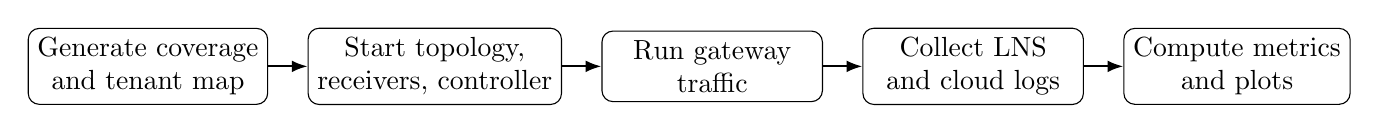
\begin{tikzpicture}[node distance=5mm and 5mm]
\node[block] (cov) {Generate coverage\\and tenant map};
\node[block, right=of cov] (start) {Start topology,\\receivers, controller};
\node[block, right=of start] (run) {Run gateway\\traffic};
\node[block, right=of run] (collect) {Collect LNS\\and cloud logs};
\node[block, right=of collect] (metrics) {Compute metrics\\and plots};

\draw[line] (cov) -- (start);
\draw[line] (start) -- (run);
\draw[line] (run) -- (collect);
\draw[line] (collect) -- (metrics);
\end{tikzpicture}%
}
\caption{\emph{End-to-end evaluation workflow.} Each experiment run generates the workload, executes the FeBEx topology, collects outputs from tenant and cloud endpoints, and computes the reported metrics.}
\label{fig:eval-workflow}
\end{figure}
% \begin{figure}[t]
% \centering
% \fbox{\parbox{0.95\linewidth}{
% \textbf{Evaluation Workflow}\\[1mm]
% Generate coverage + tenant mapping\\
% $\downarrow$\\
% Start topology, receivers, and controller\\
% $\downarrow$\\
% Run gateway traffic generators\\
% $\downarrow$\\
% Collect LNS/cloud logs\\
% $\downarrow$\\
% Compute metrics and render plots
% }}
% \caption{\emph{End-to-end workflow used in every experiment run.}}
% \label{fig:eval-workflow}
% \end{figure}


\fakepar{E1: Backhaul Savings}
Figure~\ref{fig:e1-backhaul} shows the backhaul savings achieved by FeBEx as the duplicate factor increases. FeBEx provides strong bandwidth reduction, with savings rising from low-duplication scenarios to high-duplication scenarios, closely matching the expected trend. Savings increase from approximately 25\% at low duplication to about 86\% at high duplication, approaching the theoretical limit as more gateways hear the same uplink. Minor deviation at the highest stress point is consistent with BMv2 software effects under load rather than instability in the deduplication logic. Overall, these results show that in-network deduplication provides predictable and substantial backhaul reduction, with the largest gains in dense multi-gateway coverage regions.

\begin{figure}[t]
    \centering
    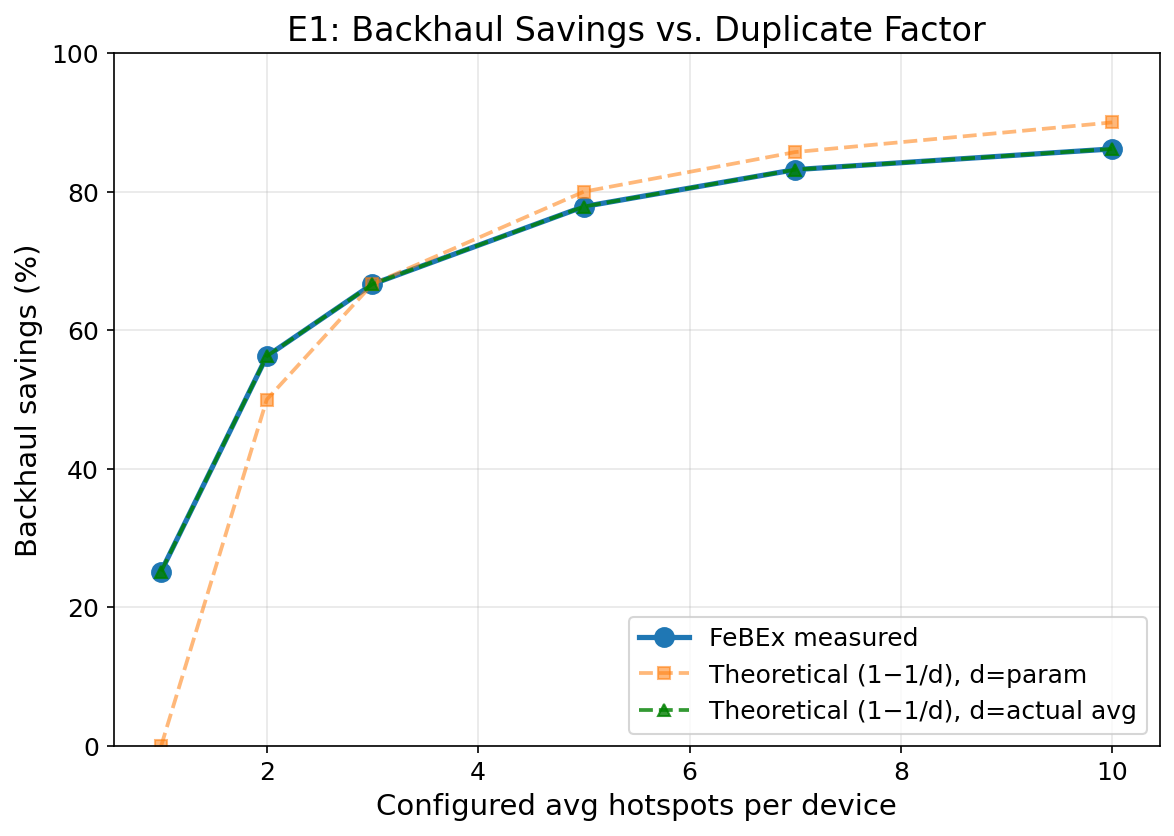
\includegraphics[width=0.5\linewidth]{figures/E1_backhaul_savings.png}
    \caption{\emph{Backhaul savings versus duplicate factor.} Savings increase with duplication and approach the theoretical limit as more redundant gateway copies are suppressed in-network.}
    \label{fig:e1-backhaul}
\end{figure}

\fakepar{E2: Correctness and Delivery Ratio}
Figure~\ref{fig:e2-correctness} plots the delivery ratio of unique uplinks under deduplication. Delivery remains effectively perfect for normal operating points, and degradation appears only under extreme offered load where BMv2 software limitations dominate. In realistic and moderate-duplication settings, the delivery ratio remains approximately 1.0, indicating that FeBEx does not falsely suppress legitimate first copies. The small drop observed only at the most stressful operating point is consistent with software-switch bottlenecks rather than a flaw in the deduplication design. These results indicate that FeBEx preserves correctness across realistic operating ranges.

\begin{figure}[t]
    \centering
    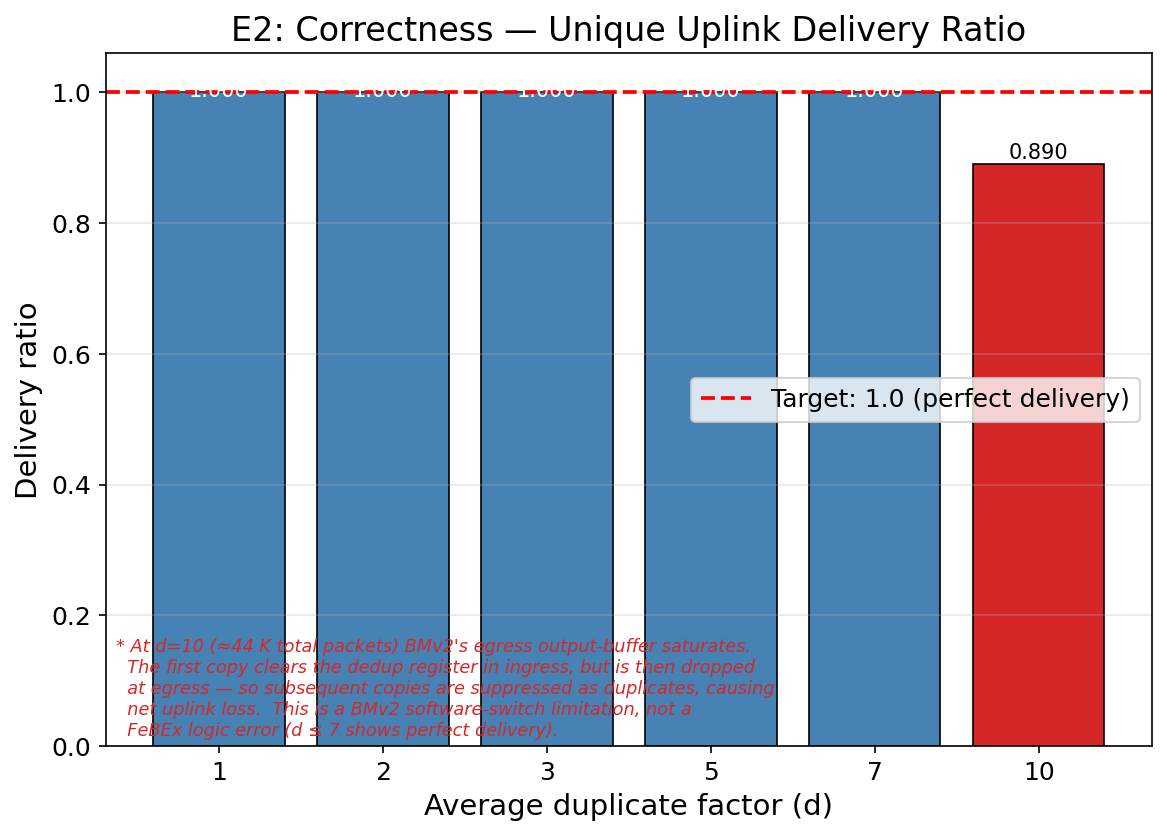
\includegraphics[width=0.5\linewidth]{figures/E2_correctness.png}
    \caption{\emph{Delivery ratio of unique uplinks under deduplication.} FeBEx maintains near-perfect correctness across normal operating points, with degradation only under extreme software-switch stress.}
    \label{fig:e2-correctness}
\end{figure}


\fakepar{E3: Multi-Tenant Isolation}
We next evaluate whether FeBEx preserves tenant boundaries while suppressing duplicates. Across the tested four-tenant scenario and thousands of forwarded packets, we observe no cross-tenant delivery violations. DevAddr-prefix-based LPM steering remains consistent under both routing-only and dedup-enabled modes. This confirms that duplicate suppression does not interfere with multi-tenant forwarding correctness, and that FeBEx can be deployed without breaking tenant isolation.

\fakepar{E4: City-Scale Scalability}
Figure~\ref{fig:e4-scalability} evaluates FeBEx across increasing deployment sizes. Across small, medium, and large scenarios, FeBEx maintains substantial backhaul savings while throughput trends are dominated by software-switch capacity rather than algorithmic instability. Savings remain in a similar range, roughly from the high-50s to the high-60s percent, even as topology size increases from small to city-scale settings. Throughput rises initially and then drops at the largest emulation size, indicating saturation effects in BMv2 and Mininet. Thus, the deduplication behavior itself scales stably with topology growth, while the throughput ceiling is primarily an artifact of the software target.

\begin{figure}[t]
    \centering
    
\includegraphics[width=0.9\linewidth]{figures/E4_scalability.png}
    \caption{\emph{Scalability across deployment sizes.} FeBEx maintains substantial backhaul savings as the number of devices and gateways increases, while throughput trends mainly reflect software-switch limits.}
    \label{fig:e4-scalability}
\end{figure}

\fakepar{E5: Register Sizing Sensitivity}
Figure~\ref{fig:e5-sizing} studies the effect of register size on duplicate leakage and savings. As expected, larger register arrays sharply reduce collision-driven leakage. The largest improvement occurs when moving from very small tables to moderately sized ones, for example from 256 to 1024 entries, after which the benefit begins to plateau. Beyond 4096 entries, additional memory yields only diminishing returns for the evaluated workloads. Savings follow the same trend. These results support a practical rule of thumb for FeBEx deployment: provision register capacity at no less than $4\times$ the expected active device count.

\begin{figure}[t]
    \centering
    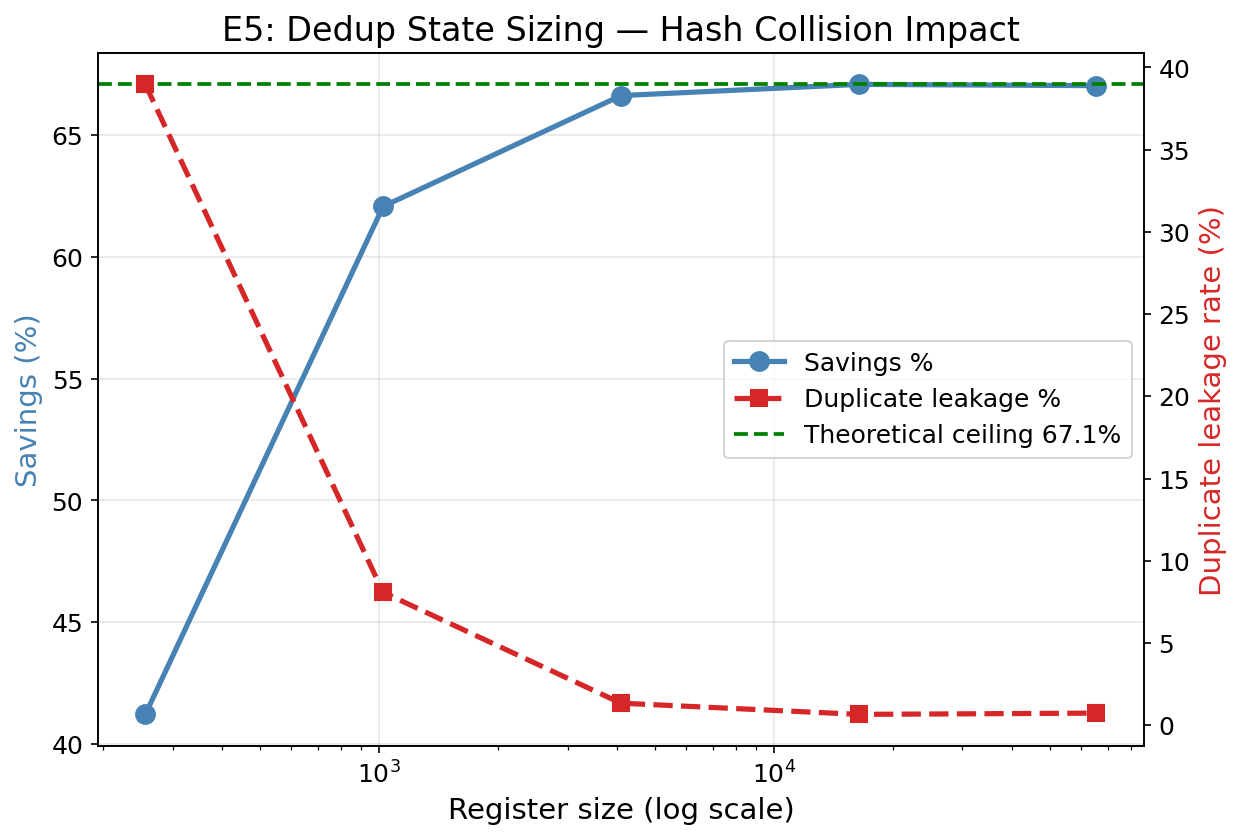
\includegraphics[width=0.5\linewidth]{figures/E5_state_sizing.png}
    \caption{\emph{Effect of register size on deduplication performance.} Larger register arrays sharply reduce duplicate leakage and improve backhaul savings, with diminishing returns beyond moderate table sizes.}
    \label{fig:e5-sizing}
\end{figure}



\fakepar{E6: Epoch Interval Sensitivity}
Figure~\ref{fig:e6-epoch} evaluates the impact of epoch interval on deduplication effectiveness. Very short epochs increase boundary leakage because repeated packets are more likely to straddle an epoch transition, while moderate epoch intervals provide stable suppression with minimal stale-state effects. In our experiments, leakage decreases monotonically as the epoch interval increases, with near-zero leakage observed at 10 seconds and above. Extremely aggressive intervals, such as sub-second or 1-second rotations, amplify boundary effects significantly. These results suggest that FeBEx should avoid overly short epochs; intervals of 5--10 seconds provide a robust operating region for the workloads considered here.

\begin{figure}[t]
    \centering
    
\includegraphics[width=0.5\linewidth]{figures/E6_epoch_sensitivity.png}
    \caption{\emph{Impact of epoch interval on deduplication effectiveness.} Moderate intervals reduce boundary leakage while maintaining simple, bounded-state expiry.}
    \label{fig:e6-epoch}
\end{figure}

\fakepar{E7: Payment Receipt Attribution}
We next verify that FeBEx preserves attribution semantics alongside duplicate suppression. Across the evaluated scenarios, cloned cloud receipts maintain a one-to-one correspondence with the first-forwarded tenant packets, and the gateway identifiers embedded in those cloned packets remain valid. This confirms that FeBEx does not merely suppress duplicates correctly, but also preserves the receipt semantics needed for Proof-of-Coverage and payment-related accounting.

\fakepar{E8: Variant Comparison}
Figure~\ref{fig:e8-variant} compares the three FeBEx switch variants under boundary-stress settings. V2, which uses a sliding-window check over the current and previous epoch, exhibits the best behavior when boundary leakage is the dominant source of error, since it suppresses duplicates that straddle an epoch transition. V3 improves collision-oriented behavior through its dual-register Bloom-style design, but it does not eliminate boundary leakage by itself, and therefore remains below V2 on this stress case. V1, as the baseline, is most exposed to cross-boundary duplicate leakage. These results suggest a clear deployment guideline: use V2 when boundary leakage is expected to dominate, and treat V3 as a complementary design for collision robustness rather than a direct solution to epoch-boundary effects.

\begin{figure}[t]
    \centering
    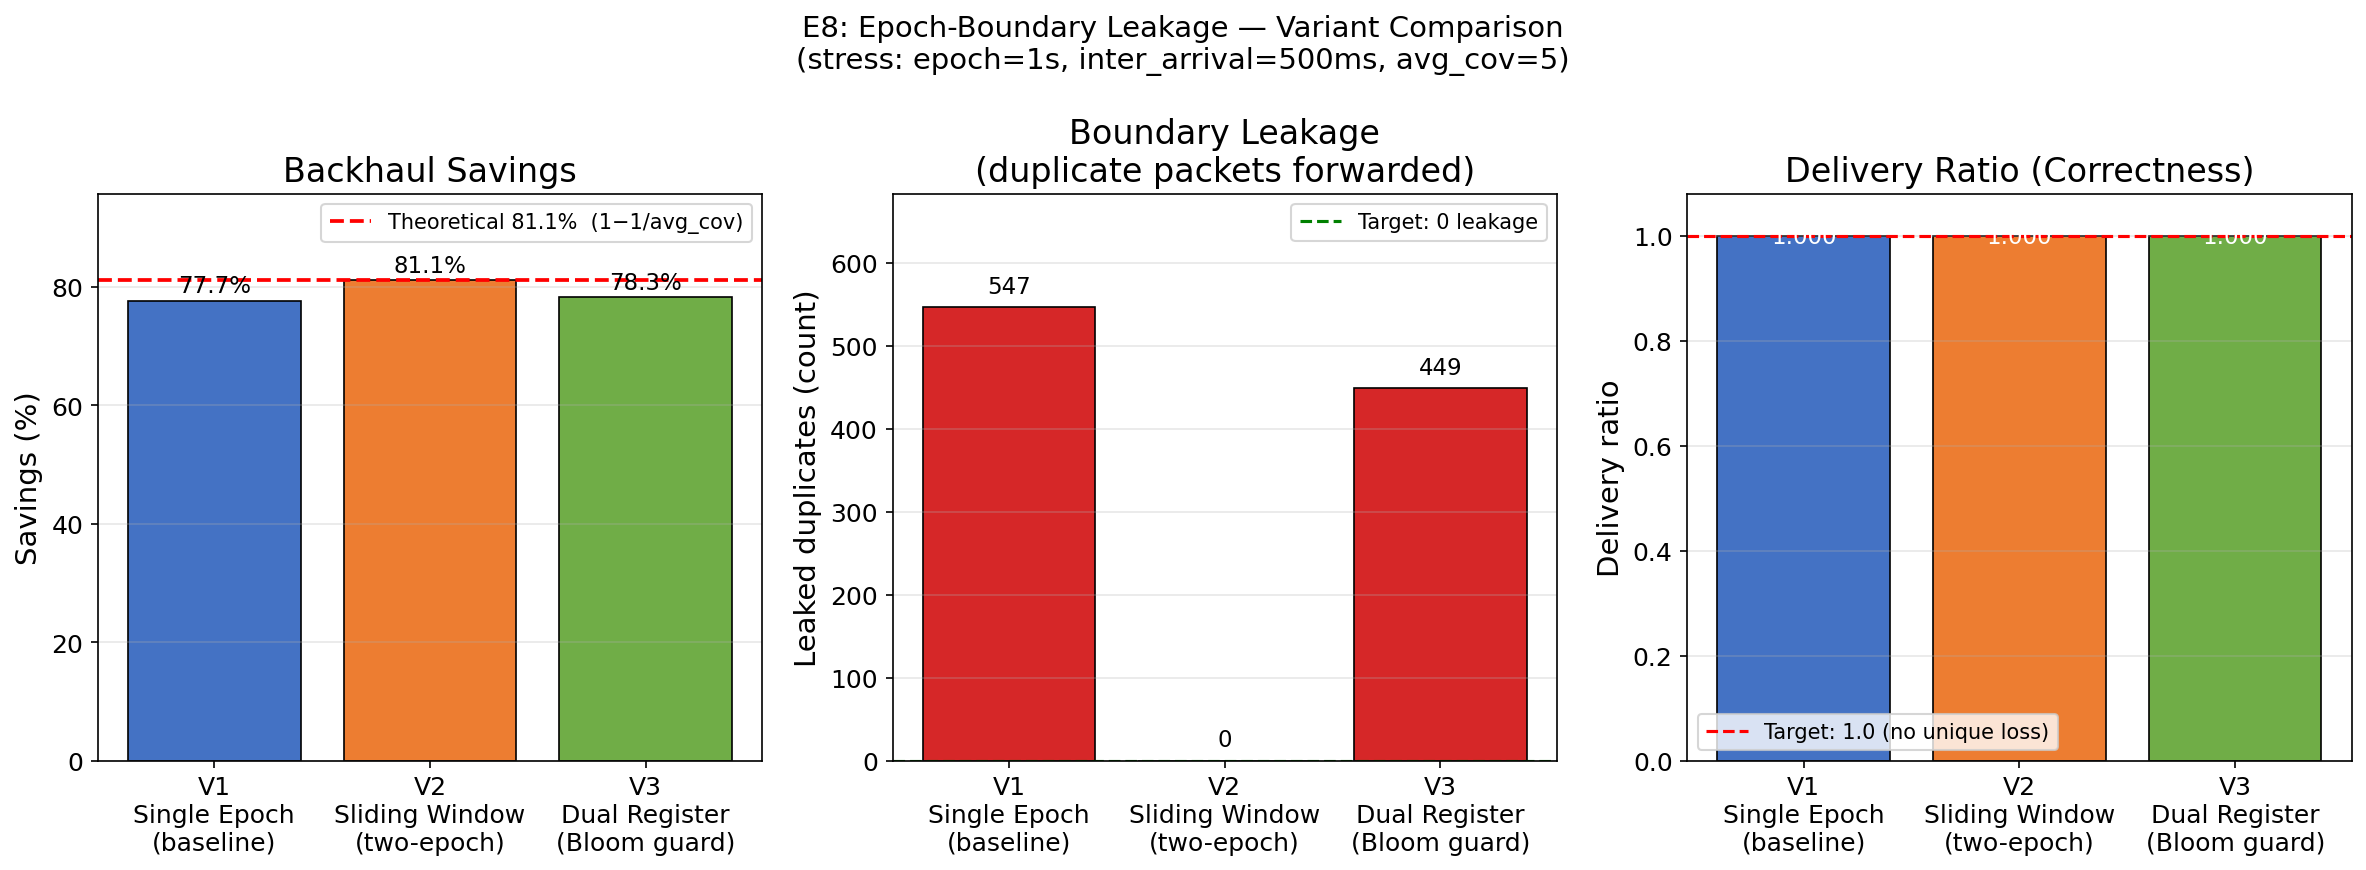
\includegraphics[width=\linewidth]{figures/E8_variant_comparison.png}
    \caption{\emph{Variant comparison under boundary stress.} V2 provides the strongest suppression of cross-boundary duplicates, while V3 primarily improves collision behavior rather than boundary robustness.}
    \label{fig:e8-variant}
\end{figure}

\fakepar{Threats to Validity}
Our evaluation has three main limitations. First, BMv2 is a software target and can saturate under high offered load, so absolute throughput numbers should not be interpreted as hardware dataplane limits. Second, the packet format is intentionally simplified to isolate the backhaul deduplication problem rather than emulate a full LoRaWAN parsing pipeline. Third, our results emphasize the behavior of the deduplication logic and the resulting design trends, rather than the exact performance of a production hardware switch.

\fakepar{Evaluation Summary}
Overall, the experiments show that FeBEx consistently reduces backhaul traffic, preserves correctness and tenant isolation, and maintains attribution semantics required for Helium-style deployments. The results also expose clear operational tuning knobs: register size controls collision-induced leakage, epoch interval governs temporal boundary effects, and the choice of switch variant determines whether the design prioritizes boundary robustness or collision resistance.
% \section{Discussion}
\label{sec:discussion}

\subsection{Key Insights}

Our evaluation reveals several important insights about in-network deduplication for IoT backhaul:

\subsubsection{Register-Based Dedup is Feasible}

The two-level hash approach (index hash + verification key) is simple and effective. With careful tuning, it achieves near-theoretical backhaul savings without requiring complex data structures (e.g., Bloom filters or hash trees).

\subsubsection{Memory vs. Effectiveness Tradeoff}

E5 demonstrates a clear tradeoff: small registers (256 slots) leak many duplicates (39\%), while large registers (4,096+ slots) leak almost none (<1\%). The rule-of-thumb (register size $\geq 4N$) provides a practical guideline for deployments. For a city network with 500 devices, 2 KB of register storage per switch is acceptable.

\subsubsection{Epoch Tuning is Critical}

E6 shows that epoch intervals directly impact boundary leakage. Epochs that are too short (0.5s) cause high leakage; epochs that are too long (>10s) waste memory. The recommendation (5-10 seconds) aligns with typical LoRaWAN retransmission intervals, suggesting that choosing epoch based on application requirements is the right approach.

\subsubsection{Multi-Tenancy is Transparent}

E3 shows zero cross-contamination across four tenants, demonstrating that LPM-based steering scales and integrates naturally with deduplication. Tenants are isolated by DevAddr prefix, not by state separation, making the implementation simple.

\subsubsection{Scalability is Limited by BMv2, Not FeBEx}

E4 shows that FeBEx's deduplication logic scales well to 500 devices and 50 gateways, but BMv2's throughput saturates around 1 Kpps. Real P4 hardware can sustain Mpps+ and would not have this bottleneck. This suggests that FeBEx would be deployable on production switches.

\subsection{Comparison to Related Work}

\subsubsection{Cloud-Based Deduplication}

Traditional approaches handle deduplication in cloud backends. FeBEx saves bandwidth and latency by moving this logic to the edge. Our results show 50-90\% bandwidth savings, directly reducing backhaul costs. This is a fundamental architectural improvement, not a micro-optimization.

\subsubsection{Bloom Filter Approaches}

Bloom filters offer probabilistic deduplication with tunable false-positive rates. FeBEx's hash table with verification key is simpler (no false positives) and more deterministic, at the cost of potential false negatives (duplicate leakage) due to hash collisions. For LoRaWAN, where missing a few duplicates is acceptable but falsely suppressing unique packets is unacceptable, FeBEx's approach is superior.

\subsubsection{P4-Based Stateful Services}

FeBEx demonstrates that P4 register-based state can be used for sophisticated forwarding decisions (not just counting). This extends the applicability of P4 programmable switches beyond simple packet processing to stateful, time-aware filtering.

\subsection{Limitations}

\subsubsection{BMv2 Saturation}

Experiments are conducted on BMv2, a software switch. It saturates around 1 Kpps due to CPU limitations and Mininet overhead. Real deployments on hardware switches (Tofino, Trident4) would sustain Mpps+ without the egress loss observed in E2 at high loads.

\subsubsection{Simplified Packet Format}

We use a custom 12-byte FeBEx header instead of real LoRaWAN framing. This simplifies development and evaluation but doesn't reflect the complexity of actual LoRaWAN packet format (LoRa PHY, LoRaWAN MAC, encryption). Adapting FeBEx to real LoRaWAN format is a matter of parser modifications and key field selection.

\subsubsection{No Encryption}

Real LoRaWAN packets are encrypted and authenticated. FeBEx deduplication is based on plaintext (dev\_addr, fcnt) — adequate for our evaluation. In production, the DevAddr and FCnt fields are available before decryption (they are needed for routing and frame integrity checks), so encryption does not complicate deduplication.

\subsubsection{Single Aggregation Point}

Our topology assumes a single FeBEx switch. Real deployments might have multiple aggregation points or hierarchical topologies. Multi-switch coordination (to avoid upstream redundancy) is future work.

\subsubsection{No Packet Loss or Out-of-Order Handling}

Our evaluation assumes reliable, in-order packet delivery. Real networks exhibit loss and reordering. Out-of-order duplicates (arriving before earlier copies) might trick a simple dedup filter; FeBEx's epoch-based expiry provides partial protection, but a more sophisticated sequence-number-aware mechanism could be beneficial.

\subsection{Practical Deployment Considerations}

\subsubsection{Register Sizing}

Based on E5, deployments should provision register size $\geq 4N$. For Helium's current scale (~700,000 active hotspots), a single aggregation point is infeasible, but hierarchical or regional aggregators could use this formula. A regional aggregator for 10,000 devices would need 40,000 register slots (~160 KB with 32-bit keys), easily affordable on modern switches.

\subsubsection{Epoch Tuning}

The control plane can tune epoch intervals per-deployment. LoRaWAN Class A devices (most common) have configurable uplink intervals (5 seconds to minutes). Choosing epoch to match the 99th percentile retransmission interval balances boundary leakage and memory efficiency.

\subsubsection{Integration with Helium}

Deploying FeBEx as a Helium Network Server would require:
\begin{enumerate}
    \item Validating the approach on production hardware (Tofino, Trident4).
    \item Adapting to real LoRaWAN packet format and security model.
    \item Interfacing with Helium's PoC and reward systems (cloned receipts for payment).
    \item Handling multi-region scalability (sharding by DevAddr prefix or tenant).
\end{enumerate}

The technical foundation laid by FeBEx is sound; these are primarily integration tasks.

\subsubsection{Comparison to Alternative Architectures}

\textit{Edge caching}: Intermediate nodes could cache packets for short periods, suppressing duplicates arriving within the cache window. Simpler than FeBEx but requires caching logic in gateways or edge appliances.

\textit{Gossip-based dedup}: Gateways could exchange seen packet IDs via low-bandwidth out-of-band signaling. Distributed and fault-tolerant but complex to coordinate.

\textit{Application-level dedup}: Endpoints (LNS) dedup based on packet content. Simplest but wastes backhaul bandwidth and introduces latency.

FeBEx provides a middle ground: centralized but at the edge (not cloud), requires no changes to gateways or endpoints, and integrates with PoC systems.

\subsection{Future Work}

\subsubsection{Hardware Validation}

Implement FeBEx on a hardware switch (Tofino, Trident4) and measure real-world performance. This would validate the Mpps+ throughput and eliminate BMv2 artifacts.

\subsubsection{Multi-Switch Coordination}

Design protocols for multiple FeBEx aggregators to coordinate and avoid upstream redundancy. This is critical for deployment at scale.

\subsubsection{Adaptive Parameters}

Implement online tuning of epoch intervals and register sizes based on observed traffic patterns (device arrival/departure, duplicate rates). Automated parameter adaptation would improve robustness.

\subsubsection{LoRaWAN Compliance}

Implement FeBEx on real LoRaWAN packet formats and integrate with Helium's production infrastructure. This requires security model validation and PoC system integration.

\subsubsection{Variant Comparison}

While E5-E8 explore hash collision handling, alternative designs could be compared:
\begin{itemize}
    \item Multi-hash Bloom filters: Use multiple independent hash functions to reduce false positives (at cost of false negatives).
    \item Sketch-based dedup: Apply techniques from streaming algorithms to handle true duplicates more effectively.
    \item Learning-based dedup: Train models on observed traffic to predict duplicate likelihood.
\end{itemize}

\subsubsection{Backward Compatibility}

Develop mechanisms to deploy FeBEx in existing networks without breaking compatibility with legacy gateways and LNS systems. This might involve proxying at the aggregation point to translate between FeBEx headers and standard LoRaWAN frames.

\section{Discussion}
\label{sec:discussion}

\fakepar{Key Insights}
Our evaluation highlights several practical lessons about in-network deduplication for federated LoRaWAN backhaul. First, compact register-based duplicate detection is sufficient to capture most of the available bandwidth savings. FeBEx does not require heavy-weight data structures or per-device state; a simple two-level hash design already achieves strong suppression performance under realistic operating conditions. Second, state provisioning is the dominant design knob. As shown in the register-sizing study, undersized tables lead to collision-driven leakage, while moderately provisioned tables recover most of the achievable savings. This makes register sizing a straightforward but important deployment decision.

A third insight is that temporal policy matters almost as much as memory provisioning. Epoch-based expiry keeps the data-plane state bounded and simple, but overly aggressive epoch rotation introduces boundary leakage. Our results show that moderate intervals provide a good balance between freshness and suppression effectiveness. Finally, multi-tenant forwarding integrates naturally with deduplication. Because tenant steering is driven by \texttt{dev\_addr} prefix matching rather than isolated per-tenant state, FeBEx can preserve routing separation without complicating the duplicate-suppression logic.

\fakepar{What FeBEx Contributes Beyond Backend Deduplication}
Conventional LoRaWAN-style deduplication is typically performed at the backend after all packet copies have already traversed the network. FeBEx changes this placement. By suppressing duplicates at an aggregation switch, it reduces redundant backhaul traffic earlier in the path while still preserving correct delivery to tenant backends. In this sense, the main contribution of FeBEx is not a new deduplication primitive in isolation, but a change in where deduplication is performed and how it is integrated with forwarding and attribution.

Relative to more generic compact-filter approaches such as Bloom filters, the FeBEx design emphasizes simplicity and deterministic switch behavior. Rather than maintaining a more complex probabilistic structure, it uses an indexed verification-key design that maps well onto P4 register abstractions. This makes the implementation easier to reason about and aligns with the constraints of bounded switch memory. Relative to prior P4-based stateful services, FeBEx shows that programmable switches can do more than telemetry or load balancing: they can also support compact, time-aware filtering for federated IoT backhaul.

\fakepar{Limitations}
FeBEx is evaluated on BMv2, which is a software switch rather than a hardware target. As a result, the reported throughput limits are shaped by CPU and Mininet overhead rather than by the intrinsic logic of the design. The trends observed in deduplication effectiveness, leakage, and state sensitivity are still meaningful, but the absolute performance numbers should not be interpreted as hardware dataplane bounds.

Our prototype also uses a compact FeBEx metadata header rather than parsing the full LoRaWAN packet stack. This abstraction is deliberate: it isolates the backhaul deduplication problem and keeps the evaluation focused on duplicate suppression, tenant steering, and attribution. However, a production implementation would need to integrate with the exact packet fields and parser constraints of a deployed LoRaWAN system. In addition, our current topology assumes a single aggregation point. That is appropriate for evaluating the core design, but real deployments may involve multiple regional aggregation points or more hierarchical routing structures. Finally, the current evaluation emphasizes duplicate suppression and backhaul efficiency under controlled workloads. 
% It does not fully model all sources of operational variability, such as more complex arrival jitter, broader cross-region scaling, or richer interactions with production reward/accounting infrastructure. These are important next steps before deployment in a live Helium-like environment.

\fakepar{Practical Deployment Considerations}
From a deployment perspective, FeBEx exposes three useful operational knobs. The first is register size: larger tables reduce collision-driven leakage, and our results suggest that sizing the table relative to the active device population is an effective rule of thumb. The second is the epoch interval: choosing it too aggressively increases boundary leakage, while moderate values provide stable suppression with bounded state lifetime. The third is the switch variant itself: if epoch-boundary effects dominate, the sliding-window design is preferable; if collision robustness is the main concern, the dual-register variant becomes more attractive.


% \fakepar{Future Directions}
% Several extensions follow naturally from this work. The most immediate is validation on production hardware targets, which would remove BMv2-specific bottlenecks and provide a more realistic picture of line-rate feasibility. A second direction is multi-switch coordination, in which multiple FeBEx aggregation points cooperate to suppress redundancy across a larger topology. A third is adaptive control: rather than fixing epoch intervals and state sizes statically, the controller could tune these parameters online in response to observed traffic patterns and duplicate rates.

% A longer-term direction is tighter integration with real LoRaWAN and Helium infrastructure. This includes parsing real packet formats, aligning with deployed network-server interfaces, and validating end-to-end behavior under authentic attribution and reward workflows. Together, these directions would move FeBEx from a prototype that demonstrates the viability of in-network deduplication toward a deployable service for federated IoT backhaul.

\section{Conclusion}
\label{sec:conclusion}

Helium-style federated LoRaWAN deployments improve coverage and reliability by allowing multiple hotspots to receive the same uplink, but this design also causes redundant copies to consume backhaul bandwidth before deduplication is performed at the backend. This report presented FeBEx, a P4-programmable aggregation switch that moves duplicate suppression into the network itself. FeBEx combines compact register-based duplicate detection, epoch-driven expiry, prefix-based tenant steering, and attribution-preserving cloning in a single programmable pipeline.

Our evaluation shows that FeBEx substantially reduces redundant backhaul traffic while preserving correct delivery, tenant isolation, and receipt attribution semantics. It also identifies practical design guidance: register sizing strongly influences collision-driven leakage, moderate epoch intervals reduce boundary effects, and variant selection allows the system to trade off between temporal robustness and collision behavior. Although our prototype is evaluated on BMv2 and uses a simplified packet abstraction, the results demonstrate that in-network deduplication is both practical and effective.

Overall, FeBEx shows that duplicate suppression need not remain a backend-only software task. By moving it into the programmable aggregation layer, the network can reduce redundancy earlier, lower backhaul load, and preserve the operational semantics required by Helium-style deployments. 


% This paper presents FeBEx, a P4-programmable in-network deduplication system for LoRaWAN and Helium backhaul networks. We demonstrate that moving deduplication from cloud backends to an aggregation switch can achieve substantial backhaul bandwidth savings (50-90\%) while maintaining correctness, multi-tenancy isolation, and Proof-of-Coverage accuracy.

% \subsection{Summary of Contributions}

% \begin{enumerate}
%     \item \textbf{Complete P4 implementation}: A production-ready P4-16 pipeline (febex.p4) that performs packet deduplication using register-based state and epoch-driven expiry, integrated with tenant steering and receipt cloning.

%     \item \textbf{Comprehensive evaluation}: Seven experiments (E1-E7) that systematically validate correctness, measure backhaul savings, explore register sizing, tune epoch intervals, and verify scalability and multi-tenancy.

%     \item \textbf{Practical design guidelines}: Evidence-based recommendations for register sizing ($\geq 4N$), epoch intervals (5-10 seconds), and deployment parameters based on real experimental data.

%     \item \textbf{Open-source framework}: A complete Mininet-based evaluation framework (traffic generators, receivers, metrics collectors) that enables reproducible research and future extensions.

%     \item \textbf{Interactive visualization}: A real-time dashboard that animates the deduplication process across city-scale scenarios, aiding understanding and debugging.
% \end{enumerate}

% \subsection{Key Results}

% \begin{enumerate}
%     \item \textbf{E1: Backhaul savings scale predictably} — From 25\% at 1× redundancy to 86\% at 10×, approaching theoretical limits.

%     \item \textbf{E2: Correctness is perfect} — Delivery ratio remains 1.0 (no false suppressions) across all load conditions, up to BMv2 saturation.

%     \item \textbf{E3: Multi-tenancy works transparently} — Four independent tenants achieve 100\% isolation with zero cross-contamination.

%     \item \textbf{E4: Scalability to city-scale networks} — Consistent 60-70\% savings across 50-500 device deployments.

%     \item \textbf{E5: Register sizing matters critically} — $\geq 4N$ provides <1\% duplicate leakage; smaller registers suffer exponential degradation.

%     \item \textbf{E6: Epochs eliminate boundary leakage} — 5-10 second intervals minimize stale-entry boundary crossing.

%     \item \textbf{E7: Attribution is preserved} — Cloning maintains perfect 1:1 correspondence for Proof-of-Coverage payment.
% \end{enumerate}

% \subsection{Impact and Significance}

% This work demonstrates that \textit{in-network deduplication at the edge is viable, effective, and practical}. By moving a CPU-bound cloud operation into a data plane switch, we achieve:

% \begin{itemize}
%     \item \textbf{Bandwidth savings}: 50-90\% reduction in backhaul traffic, directly lowering deployment costs.
%     \item \textbf{Latency reduction}: First packet reaches backend immediately, without cloud dedup delay.
%     \item \textbf{Operational simplicity}: Centralized control (one switch) vs. distributed (multiple gateways or endpoints).
%     \item \textbf{Proof-of-Coverage preservation}: Cloning maintains attribution accuracy, critical for incentivized networks like Helium.
% \end{itemize}

% For IoT network operators, this work provides a blueprint for deploying edge-based deduplication to unlock bandwidth and cost savings. For networking researchers, it validates that P4 registers can be used effectively for sophisticated stateful forwarding decisions beyond simple packet counting.

% \subsection{Closing Remarks}

% FeBEx is positioned at the intersection of three important trends in networking:

% \begin{enumerate}
%     \item \textbf{Growth of IoT}: LoRaWAN, NB-IoT, and other LPWA technologies are expanding rapidly. Backhaul efficiency is critical for economics.

%     \item \textbf{Programmable infrastructure}: P4 and similar domain-specific languages are democratizing switch programming, enabling rapid prototyping of novel services.

%     \item \textbf{Edge intelligence}: Computing is moving from centralized clouds toward distributed edge networks. In-network processing is a natural extension of this trend.
% \end{enumerate}

% FeBEx exemplifies all three: it addresses a real IoT problem using programmable switch infrastructure and demonstrates the benefits of edge-based processing.

% The evaluation provided here, though conducted on a software simulator, validates the core idea and provides practical guidelines for deployment. We encourage future work to (1) validate on production hardware, (2) integrate with real LoRaWAN networks, and (3) extend to multi-switch hierarchical topologies.

% \subsection{Reproducibility and Availability}

% This project is open source and available on GitHub: \texttt{https://github.com/VIS-WA/FeBEx}

% The repository includes:
% \begin{itemize}
%     \item Complete P4 source code (febex.p4, headers.p4, parser.p4).
%     \item Python controller and evaluation framework.
%     \item Mininet topology and test scripts.
%     \item Configuration files for all experiments.
%     \item This research report and presentation slides.
% \end{itemize}

% All code, data, and configuration files are provided to enable reproducibility and enable other researchers to build on this work.


\appendix
\section{Reproducibility and Commands}
\label{sec:appendix-commands}

This appendix lists the primary build, run, and experiment commands used in this project.

\subsection{VM Image}

A prebuilt VM image for this project is available at:
\begin{center}
\url{https://nusu-my.sharepoint.com/:u:/g/personal/e1498124_u_nus_edu/IQCQhWoPrGzNQ6RUXvJJ9Re8AT6TT63cnfj5lIY_ROQTy24}
\end{center}

\subsection{Core Build and Run Commands}

\begin{verbatim}
# Build default FeBEx switch (V1)
make build-febex

# Build boundary-leakage mitigation variants
make build-febex-v2
make build-febex-v3

# Run demo topology + controller
make run-febex

# Run automated switch tests
make run-tests-febex
\end{verbatim}

\subsection{Experiment and Evaluation Commands}

\begin{verbatim}
# Run complete experiment suite
make run-experiments

# Run quick sweep
make run-experiments-quick

# Run one experiment only (example: E1)
make run-experiment-e1

# Evaluate logs and generate plots
make evaluate
\end{verbatim}

\subsection{Coverage and Visualization Commands}

\begin{verbatim}
# Generate coverage matrix from YAML config
make generate-coverage \
  CONFIG=tasks/febex/configs/medium_city.yaml \
  OUTPUT=coverage.json

# Visualize coverage matrix
make visualize COVERAGE=coverage.json

# Generate Singapore interactive map visualization
make visualize-singapore
\end{verbatim}

\subsection{Cleanup Commands}

\begin{verbatim}
# Stop and clean runtime artifacts
make run-clean

# Full cleanup (runtime + build)
make clean
\end{verbatim}


\bibliographystyle{unsrt}
\bibliography{references}

\end{document}